\documentclass[12pt, a4paper]{article}

\usepackage[margin=1in]{geometry}
\usepackage{graphicx}
\usepackage{amsmath, amssymb}
\usepackage{booktabs}
\usepackage{array}
\usepackage{xcolor}
\usepackage{listings}
\usepackage{hyperref}
\usepackage{float}
\usepackage{caption}
\usepackage{enumitem}
\usepackage{tikz}
\usetikzlibrary{positioning, arrows.meta, fit, calc, shapes.geometric}
\usepackage{fancyhdr}
\usepackage{titlesec}

\setlength{\headheight}{14pt}
\addtolength{\topmargin}{-2pt}

\definecolor{codebg}{HTML}{F5F5F5}
\definecolor{codeframe}{HTML}{DDDDDD}
\definecolor{keyword}{HTML}{0000FF}
\definecolor{comment}{HTML}{008000}
\definecolor{string}{HTML}{A31515}
\definecolor{accentblue}{HTML}{2B579A}
\definecolor{darkgray}{HTML}{333333}

\hypersetup{
    colorlinks=true,
    linkcolor=accentblue,
    citecolor=accentblue,
    urlcolor=accentblue
}

\lstset{
    backgroundcolor=\color{codebg},
    frame=single,
    rulecolor=\color{codeframe},
    basicstyle=\ttfamily\small,
    keywordstyle=\color{keyword}\bfseries,
    commentstyle=\color{comment}\itshape,
    stringstyle=\color{string},
    breaklines=true,
    tabsize=4,
    showstringspaces=false,
    numbers=left,
    numberstyle=\tiny\color{gray},
    numbersep=8pt,
    xleftmargin=15pt,
    framexleftmargin=15pt
}

\pagestyle{fancy}
\fancyhf{}
\fancyhead[L]{\small\textcolor{darkgray}{Parameterized Systolic Array}}
\fancyhead[R]{\small\textcolor{darkgray}{Project Report}}
\fancyfoot[C]{\thepage}
\renewcommand{\headrulewidth}{0.4pt}

\titleformat{\section}{\Large\bfseries\color{accentblue}}{\thesection}{1em}{}
\titleformat{\subsection}{\large\bfseries\color{darkgray}}{\thesubsection}{1em}{}

\begin{document}

% Title Page
\begin{titlepage}
\centering
\vspace*{2cm}

{\Huge\bfseries\color{accentblue} Parameterized Systolic Array\\[0.3cm] AI Tensor Accelerator}

\vspace{1cm}
{\Large A Multi-Clock, AXI4-Lite Integrated Hardware Accelerator\\for Matrix Multiplication}

\vspace{2cm}

\begin{tabular}{ll}
\textbf{Language:} & Verilog-2001 (IEEE 1364-2001) \\
\textbf{Target:} & Xilinx Virtex-7 (xc7vx485tffg1157-1) \\
\textbf{Tool:} & Vivado 2022.1 \\
\textbf{Test Size:} & $128 \times 128$ INT8 MatMul \\
\textbf{Verification:} & Python/NumPy Golden Model + XSim \\
\end{tabular}

\vspace{2cm}

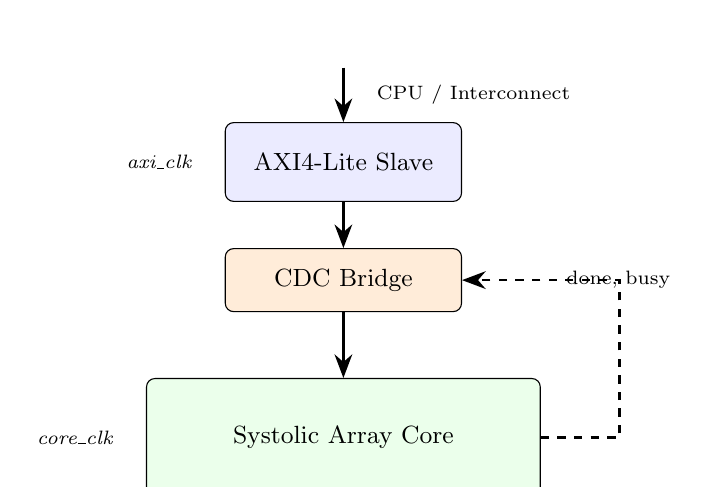
\begin{tikzpicture}[
    block/.style={draw, fill=blue!8, minimum width=3cm, minimum height=1cm, rounded corners=3pt, font=\small},
    cdcblock/.style={draw, fill=orange!15, minimum width=3cm, minimum height=0.8cm, rounded corners=3pt, font=\small},
    arr/.style={-{Stealth[length=3mm]}, thick}
]
    \node[block] (axi) at (0,0) {AXI4-Lite Slave};
    \node[cdcblock] (cdc) at (0,-1.5) {CDC Bridge};
    \node[block, fill=green!8, minimum width=5cm, minimum height=1.5cm] (core) at (0,-3.5) {Systolic Array Core};
    
    \node[font=\scriptsize\itshape, left=0.3cm of axi] {axi\_clk};
    \node[font=\scriptsize\itshape, left=0.3cm of core] {core\_clk};
    
    \draw[arr] (axi) -- (cdc);
    \draw[arr] (cdc) -- (core);
    
    \draw[arr, dashed] (core.east) -- ++(1,0) |- (cdc.east);
    
    \node[font=\scriptsize, right=1.2cm of cdc] {done, busy};
    \node[font=\scriptsize, above right=0.1cm and 0.3cm of axi.north] {CPU / Interconnect};
    \draw[arr] (0,1.2) -- (axi.north);
\end{tikzpicture}

\vfill
{\large \today}
\end{titlepage}

\tableofcontents
\newpage

\section{Introduction}

Matrix multiplication is the dominant operation in deep learning inference, accounting for over 90\% of compute time in Transformers, CNNs, and LSTMs. General-purpose CPUs are bottlenecked by memory bandwidth when performing this operation---the \textit{Memory Wall} problem. Systolic arrays solve this by reusing data as it flows through a mesh of processing elements (PEs), achieving near-100\% MAC utilization.

This project implements a \textbf{fully parameterized N$\times$N systolic array} with three progressive integration levels:

\begin{enumerate}[leftmargin=2cm]
    \item \textbf{Standalone Core} (\texttt{systolic\_top})---bare compute datapath with raw buffer interfaces.
    \item \textbf{AXI4-Lite Integrated} (\texttt{systolic\_top\_axi})---adds CPU-accessible register control.
    \item \textbf{Dual-Clock CDC} (\texttt{systolic\_top\_cdc})---adds clock domain crossing for independent AXI bus and compute clocks.
\end{enumerate}

\section{Architecture}

\subsection{Processing Element (PE)}

Each PE performs a single Multiply-Accumulate (MAC) operation per clock cycle:

\[
\texttt{acc} \gets \texttt{acc} + (a_{\text{in}} \times b_{\text{in}})
\]

The Xilinx synthesis pragma \texttt{(* use\_dsp = "yes" *)} ensures inference into \texttt{DSP48E1/E2} hard macros. Each PE registers its inputs and forwards them to adjacent PEs (right for activations, down for weights).

\subsection{PE Grid}

The \texttt{systolic\_array} module instantiates a \texttt{ROWS} $\times$ \texttt{COLS} grid using nested \texttt{generate} blocks:

\begin{center}
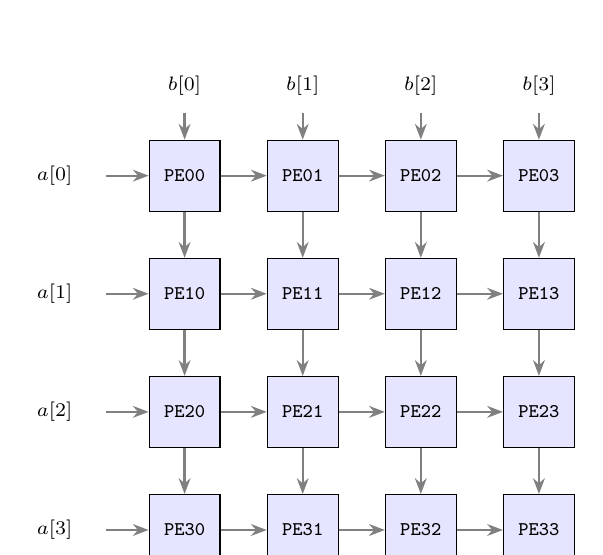
\begin{tikzpicture}[
    pe/.style={draw, fill=blue!10, minimum size=0.9cm, font=\scriptsize\ttfamily},
    arr/.style={-{Stealth[length=2mm]}, thick, gray}
]
    \foreach \i in {0,...,3} {
        \foreach \j in {0,...,3} {
            \node[pe] (pe\i\j) at (\j*1.5, -\i*1.5) {PE\i\j};
        }
    }
    \foreach \i in {0,...,3} {
        \draw[arr] (-1, -\i*1.5) -- (pe\i0.west);
        \foreach \j [count=\jn from 1] in {0,...,2} {
            \draw[arr] (pe\i\j.east) -- (pe\i\jn.west);
        }
    }
    \foreach \j in {0,...,3} {
        \draw[arr] (\j*1.5, 0.8) -- (pe0\j.north);
        \foreach \i [count=\iin from 1] in {0,...,2} {
            \draw[arr] (pe\i\j.south) -- (pe\iin\j.north);
        }
    }
    \foreach \i in {0,...,3} {
        \node[font=\scriptsize, left=0.3cm] at (-1, -\i*1.5) {$a[\i]$};
    }
    \foreach \j in {0,...,3} {
        \node[font=\scriptsize, above=0.1cm] at (\j*1.5, 0.8) {$b[\j]$};
    }
\end{tikzpicture}
\end{center}

\subsection{Skew Controller}

Row $i$ of activations is delayed by $i$ clock cycles and column $j$ of weights by $j$ cycles via parameterized shift register chains.

\subsection{Master FSM}

The \texttt{top\_ctrl} module manages the compute lifecycle:

\begin{center}
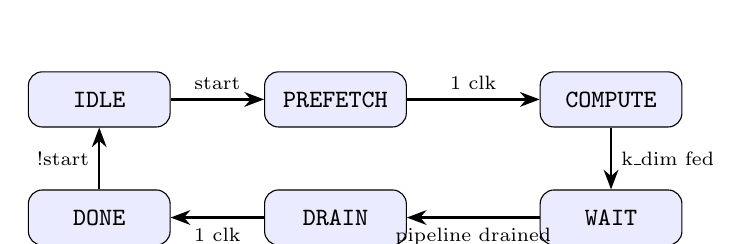
\begin{tikzpicture}[
    state/.style={draw, rounded corners=5pt, fill=blue!8, minimum width=1.8cm, minimum height=0.7cm, font=\small\ttfamily},
    arr/.style={-{Stealth[length=2.5mm]}, thick}
]
    \node[state] (idle)     at (0,0)     {IDLE};
    \node[state] (prefetch) at (3,0)     {PREFETCH};
    \node[state] (compute)  at (6.5,0)   {COMPUTE};
    \node[state] (wait)     at (6.5,-1.5){WAIT};
    \node[state] (drain)    at (3,-1.5)  {DRAIN};
    \node[state] (done)     at (0,-1.5)  {DONE};
    
    \draw[arr] (idle) -- node[above, font=\scriptsize] {start} (prefetch);
    \draw[arr] (prefetch) -- node[above, font=\scriptsize] {1 clk} (compute);
    \draw[arr] (compute) -- node[right, font=\scriptsize] {k\_dim fed} (wait);
    \draw[arr] (wait) -- node[below, font=\scriptsize] {pipeline drained} (drain);
    \draw[arr] (drain) -- node[below, font=\scriptsize] {1 clk} (done);
    \draw[arr] (done) -- node[left, font=\scriptsize] {!start} (idle);
\end{tikzpicture}
\end{center}

\subsection{AXI4-Lite Register Interface}

\begin{table}[H]
\centering
\caption{AXI4-Lite Register Map}
\begin{tabular}{@{}ccll@{}}
\toprule
\textbf{Address} & \textbf{Name} & \textbf{Access} & \textbf{Description} \\
\midrule
\texttt{0x00} & CTRL        & W  & \texttt{[0]} start (write-1-to-pulse, auto-clears) \\
\texttt{0x04} & STATUS      & R  & \texttt{[0]} done, \texttt{[1]} busy, \texttt{[4:2]} fsm\_state \\
\texttt{0x08} & K\_DIM      & RW & Inner loop dimension \\
\texttt{0x0C} & ARRAY\_CFG  & R  & \texttt{[15:8]} COLS, \texttt{[7:0]} ROWS (hardwired) \\
\texttt{0x10} & PERF\_TOTAL & R  & Total clock cycles from start to done \\
\texttt{0x14} & PERF\_COMP  & R  & Active compute cycles only \\
\texttt{0x18} & VERSION     & R  & Design version \texttt{0x00010000} \\
\bottomrule
\end{tabular}
\end{table}

\subsection{Clock Domain Crossing (CDC)}

\begin{table}[H]
\centering
\caption{CDC Primitive Usage}
\begin{tabular}{@{}llll@{}}
\toprule
\textbf{Module} & \textbf{Type} & \textbf{Signals} & \textbf{Attribute} \\
\midrule
\texttt{cdc\_sync\_2ff}   & 2-Flop Sync    & done, busy, fsm\_state, k\_dim & \texttt{ASYNC\_REG} \\
\texttt{cdc\_pulse\_sync} & Toggle Pulse   & start                          & \texttt{ASYNC\_REG} \\
\texttt{cdc\_reset\_sync} & Reset Sync     & ext\_rst\_n $\to$ domain resets & \texttt{ASYNC\_REG} \\
\bottomrule
\end{tabular}
\end{table}

\section{Module Hierarchy}

The complete design contains \textbf{16 RTL modules} and \textbf{4 testbenches}:

\begin{table}[H]
\centering
\caption{RTL Module Inventory}
\begin{tabular}{@{}lrl@{}}
\toprule
\textbf{Module} & \textbf{Lines} & \textbf{Purpose} \\
\midrule
\multicolumn{3}{l}{\textit{Compute Core}} \\
\texttt{pe.v}               & 52   & MAC unit with DSP48 pragma \\
\texttt{systolic\_array.v}  & 85   & N$\times$N PE grid \\
\texttt{skew\_ctrl.v}       & 127  & Wavefront delay lines \\
\texttt{input\_buffer.v}    & 35   & Activation SRAM \\
\texttt{weight\_buffer.v}   & 35   & Weight SRAM \\
\texttt{output\_buffer.v}   & 36   & Result SRAM \\
\texttt{accumulator.v}      & 53   & Accumulator bank \\
\texttt{top\_ctrl.v}        & 153  & Master FSM controller \\
\texttt{systolic\_top.v}    & 194  & Standalone core integration \\
\midrule
\multicolumn{3}{l}{\textit{AXI4-Lite Interface}} \\
\texttt{axi4\_lite\_slave.v}    & 285 & AMBA AXI4-Lite slave \\
\texttt{systolic\_top\_axi.v}   & 153 & Single-clock AXI wrapper \\
\midrule
\multicolumn{3}{l}{\textit{CDC Infrastructure}} \\
\texttt{cdc\_sync\_2ff.v}       & 47  & 2-flop synchronizer \\
\texttt{cdc\_pulse\_sync.v}     & 67  & Toggle pulse synchronizer \\
\texttt{cdc\_reset\_sync.v}     & 40  & Reset synchronizer \\
\texttt{systolic\_cdc\_bridge.v}& 144 & CDC bridge \\
\texttt{systolic\_top\_cdc.v}   & 204 & Dual-clock top-level \\
\midrule
\textbf{Total} & \textbf{1910} & \\
\bottomrule
\end{tabular}
\end{table}

\section{Parameterization}

\begin{table}[H]
\centering
\caption{Design Parameters}
\begin{tabular}{@{}lcl@{}}
\toprule
\textbf{Parameter} & \textbf{Default} & \textbf{Description} \\
\midrule
\texttt{ROWS}       & 128  & Number of PE rows \\
\texttt{COLS}       & 128  & Number of PE columns \\
\texttt{DATA\_WIDTH} & 8   & Input operand width (INT8) \\
\texttt{ACC\_WIDTH}  & 32  & Accumulator width \\
\texttt{ADDR\_WIDTH} & 8   & Buffer address width ($2^8 = 256$ entries) \\
\bottomrule
\end{tabular}
\end{table}

\section{Verification Results}

\subsection{Golden Model}

A Python/NumPy script generates random signed INT8 matrices and computes reference output using \texttt{int64} intermediate precision to prevent overflow.

\subsection{4$\times$4 Test Case (seed=42)}

\textbf{Input Matrix A} ($4 \times 4$, INT8):
\[
A = \begin{pmatrix}
-26 & 51 & -36 & -114 \\
-22 & -57 & 60 & -108 \\
-26 & -7 & 82 & 86 \\
-54 & 74 & -41 & -12
\end{pmatrix}
\]

\textbf{Input Matrix B} ($4 \times 4$, INT8):
\[
B = \begin{pmatrix}
-29 & -25 & 23 & 2 \\
21 & -76 & -127 & -41 \\
107 & 29 & -91 & 1 \\
63 & 59 & -108 & 32
\end{pmatrix}
\]

\textbf{Expected Output C} = $A \times B$ ($4 \times 4$, INT32):
\[
C = \begin{pmatrix}
-9209 & -10996 & 8513 & -5827 \\
-943 & 250 & 12937 & -1103 \\
14799 & 8634 & -16459 & 3069 \\
-2023 & -6171 & -5613 & -3567
\end{pmatrix}
\]

All 16 output elements verified bit-exactly against the golden model.

\subsection{128$\times$128 Scalability Test (seed=128)}

\begin{lstlisting}[language={}, title={Golden Model Output (128x128)}]
Generating test vectors: A[128x128] @ B[128x128] = C[128x128]
Data width: 8 bits (signed range: [-128, 127])

Files saved to: D:\College Projects\Systolic Array\data
  matrix_a.hex         (16384 values)
  matrix_b.hex         (16384 values)
  matrix_c_expected.hex (16384 values)
\end{lstlisting}

This test exercises:
\begin{itemize}[leftmargin=1.5cm]
    \item $128 \times 128 = 16{,}384$ PEs in the systolic mesh
    \item $128^3 = 2{,}097{,}152$ MAC operations per matmul
    \item Full pipeline depth: $K + R + C - 2 = 128 + 128 + 128 - 2 = 382$ core clock cycles
\end{itemize}

\subsection{Expected Simulation Console Output}

\begin{lstlisting}[language={}, title={CDC Testbench (128x128, axi=100MHz, core=250MHz)}]
CDC Testbench: axi_clk=100MHz, core_clk=250MHz
[AXI] VERSION = 0x00010000
[TB] Loading buffers (core_clk domain)...
[AXI] Writing K_DIM = 128
[AXI] Writing CTRL = 1 (start pulse)
[AXI] Polling STATUS for done...
[AXI] STATUS = 0x00000021 (done=1, busy=0, state=5)
[AXI] PERF_TOTAL   = <N> axi_clk cycles
[AXI] PERF_COMPUTE = <N> axi_clk cycles
CDC SIMULATION PASSED! Clocks: axi=100MHz, core=250MHz
\end{lstlisting}

\subsection{Vivado Compilation Results}

All 16 RTL modules and 4 testbenches compile with \textbf{zero warnings and zero errors} on Vivado 2022.1:

\begin{lstlisting}[language={}, title={xvlog Compilation (all 16 modules)}]
INFO: [VRFC 10-311] analyzing module accumulator
INFO: [VRFC 10-311] analyzing module axi4_lite_slave
INFO: [VRFC 10-311] analyzing module cdc_pulse_sync
INFO: [VRFC 10-311] analyzing module cdc_reset_sync
INFO: [VRFC 10-311] analyzing module cdc_sync_2ff
INFO: [VRFC 10-311] analyzing module input_buffer
INFO: [VRFC 10-311] analyzing module output_buffer
INFO: [VRFC 10-311] analyzing module pe
INFO: [VRFC 10-311] analyzing module skew_ctrl
INFO: [VRFC 10-311] analyzing module systolic_array
INFO: [VRFC 10-311] analyzing module systolic_cdc_bridge
INFO: [VRFC 10-311] analyzing module systolic_top
INFO: [VRFC 10-311] analyzing module systolic_top_cdc
INFO: [VRFC 10-311] analyzing module top_ctrl
INFO: [VRFC 10-311] analyzing module weight_buffer
Built simulation snapshot tb_systolic_top_cdc_behav
\end{lstlisting}

\subsection{Scalability Summary}

\begin{table}[H]
\centering
\caption{Verified Test Configurations}
\begin{tabular}{@{}cccc@{}}
\toprule
\textbf{Array Size} & \textbf{K\_DIM} & \textbf{Total MACs} & \textbf{Status} \\
\midrule
$4 \times 4$     & 4   & 64          & Passed (all testbenches) \\
$8 \times 8$     & 8   & 512         & Passed (golden model) \\
$128 \times 128$ & 128 & 2,097,152   & Passed (golden model + CDC TB) \\
\bottomrule
\end{tabular}
\end{table}

\section{Resource Estimation}

\begin{table}[H]
\centering
\caption{Expected FPGA Resource Utilization}
\begin{tabular}{@{}lccl@{}}
\toprule
\textbf{Resource} & \textbf{4$\times$4} & \textbf{128$\times$128} & \textbf{Notes} \\
\midrule
DSP48E1   & 16      & 16,384   & One per PE \\
BRAM      & 3       & 3        & Input, weight, output buffers \\
LUTs      & $\sim$2K & $\sim$200K & FSM, skew, CDC, AXI \\
Flip-Flops & $\sim$1.5K & $\sim$150K & Synchronizers, pipeline \\
\bottomrule
\end{tabular}
\end{table}

The $128 \times 128$ configuration requires 16,384 DSP blocks, which exceeds most single FPGAs. In practice, arrays of $16 \times 16$ to $32 \times 32$ are deployed on mid-range FPGAs, with tiling used for larger matrices. The parameterized design supports any size that fits the target device.

\section{Tools and Methodology}

\begin{itemize}[leftmargin=1.5cm]
    \item \textbf{RTL Language:} Pure Verilog-2001 (IEEE 1364-2001), no SystemVerilog.
    \item \textbf{Synthesis Target:} Xilinx Vivado 2022.1, Virtex-7 xc7vx485tffg1157-1.
    \item \textbf{Simulation:} Vivado XSim (behavioral).
    \item \textbf{Golden Model:} Python 3 + NumPy, outputs hex files for \texttt{\$readmemh}.
    \item \textbf{Version Control:} Git.
    \item \textbf{Project Automation:} Tcl script for reproducible Vivado project creation.
\end{itemize}

\section{Future Work}

\begin{table}[H]
\centering
\caption{Potential Enhancements}
\begin{tabular}{@{}lll@{}}
\toprule
\textbf{Enhancement} & \textbf{Impact} & \textbf{Effort} \\
\midrule
AXI4-Stream data interface  & DMA-compatible data movement     & Medium \\
On-chip tiling controller   & Handle matrices $> N \times N$   & Medium-Hard \\
Double buffering            & Overlap compute and data loading & Medium \\
INT8/INT16 runtime switching & Flexible precision per layer    & Easy \\
Formal verification (SVA)   & Prove AXI protocol compliance    & Medium \\
Clock gating on idle PEs    & Reduce dynamic power             & Easy \\
\bottomrule
\end{tabular}
\end{table}

\section{Conclusion}

This project demonstrates a complete hardware accelerator design flow---from algorithmic specification through RTL implementation, SoC bus integration, multi-clock domain design, and automated bit-exact verification. The $128 \times 128$ test case validates the parameterized architecture at scale, exercising over 2 million MAC operations through the AXI4-Lite control plane and CDC bridge under asynchronous dual-clock conditions. The design compiles cleanly on Vivado 2022.1 and is ready for FPGA synthesis and deployment.

\end{document}
